\section{Pipelining the ESP LLC}
\label{sec:llcImplementations}
\subsection{Original LLC}
The original LLC is implemented as a multi-cycle datapath for handling requests
according to the extended MESI protocol. The multi-cycle datapath consists of
six stages, and an FSM manages the execution of a single request across these
six stages.  In any given cycle, only one stage of the datapath is active. For
example, the first stage, which prioritizes and accepts the incoming requests,
is idle while later stages of the datapath are operating. This means that only
one request is processed by the LLC at a time, which can create backpressure
on the NoC if many requests arrive in a short time. The microarchitecture for 
this implementation is shown in Figure \ref{fig:original_muarc}.
\subsection{Pipelined LLC}
In this work, we took the existing six-stage datapath and enabled the pipelined
execution of requests. We use the same six stages from the multicycle datapath
and add pipeline registers in between each stage and logic for exerting backpressure
between individual stages. The FSM that governs the execution of an individual request
is removed, and all stages can be active in any given cycle. This implementation allows
for the simultaneous processing of multiple requests. The microarchitecture for 
this implementation is shown in Figure \ref{fig:pipeline_muarc}.

\par Pipelining a multi-cycle datapath presents numerous challenges. Signals
from previous stages that would previously stay constant throughout the
lifetime of a request now can be overwritten by new requests. This required
significant refactoring of the RTL to pass these signals with each request
through the pipeline.

\par The cache itself is a multi-bank, multi-port memory that allows for an
entire set to be read in a single clock cycle. This applies to the cache lines
themselves and also their associated metadata. Another key challenge is
avoiding read-after-write (RAW) hazards and read/write collisions within a
particular set.  RAW hazards can occur because the memory is not updated until
the final pipeline stage, while it is read in the second stage. Without careful
consideration, it would be possible for a new request to read information about
a set before an old request updates the data. It is also necessary to avoid
reading and writing the same location in this memory during the same clock
cycle to avoid non-determinism in accesses. To solve these two hazards, we introduce
a \emph{set table}, which keeps track of the sets of all requests currently active
in the pipeline. The second stage of the pipeline checks the set table before accepting
new requests in order to avoid multiple requests to the same set in flight at once. The final
pipeline stage removes an entry from the set table when it is retired. Requests
in different sets do not face these hazards, but they pose a different problem:
the memory architecture of the original LLC was not designed for simultaneous
reading and writing; we expanded the number of ports in the memory to sustain
higher throughput.

\par Pipelining the multi-cycle datapath also introduced potential for
undesired out-of-order completion of requests. There are two problematic cases:
when the LLC wants to recall an Exclusive or Modified cache line from an L2 for
eviction and when there is a cache line in a transient state waiting for a data
response from an L2. In both cases, the LLC should not service any newer
requests until the data response from the L2 has been received and completely
serviced. However, these behaviors are only determined at the fifth stage of
the pipeline, and so new requests can enter the pipeline before the response is
received.

Our solution was to add a feature to the fifth stage that stalls the first
stage and flushes all the newer requests in the pipeline into a FIFO. After the
data response has been received and serviced, the LLC will process the requests
in the FIFO before accepting any new requests from externally.
LLC will then prioritize feeding requests from the FIFO back into the pipeline
once the data response has been received and serviced.

\par While the original LLC significantly improved DMA latency for accelerators
by potentially eliminating off-chip memory accesses, the pipelined LLC
further improves DMA performance. Large DMA requests span multiple
cache lines, and the LLC handles each cache line as a separate
"request" for a different address. The pipelined LLC is designed to generate a
new "request" to insert into the second pipeline stage every cycle, allowing
the DMA request to fully utilize all stages of the pipeline. When the accelerator
data resides in the LLC, this allows a new cache line to be sent or written every
cycle, as opposed to every six cycles in the old implementation.


\begin{figure*}[t]
    \centering
    \captionsetup{justification=centering, format=hang}
    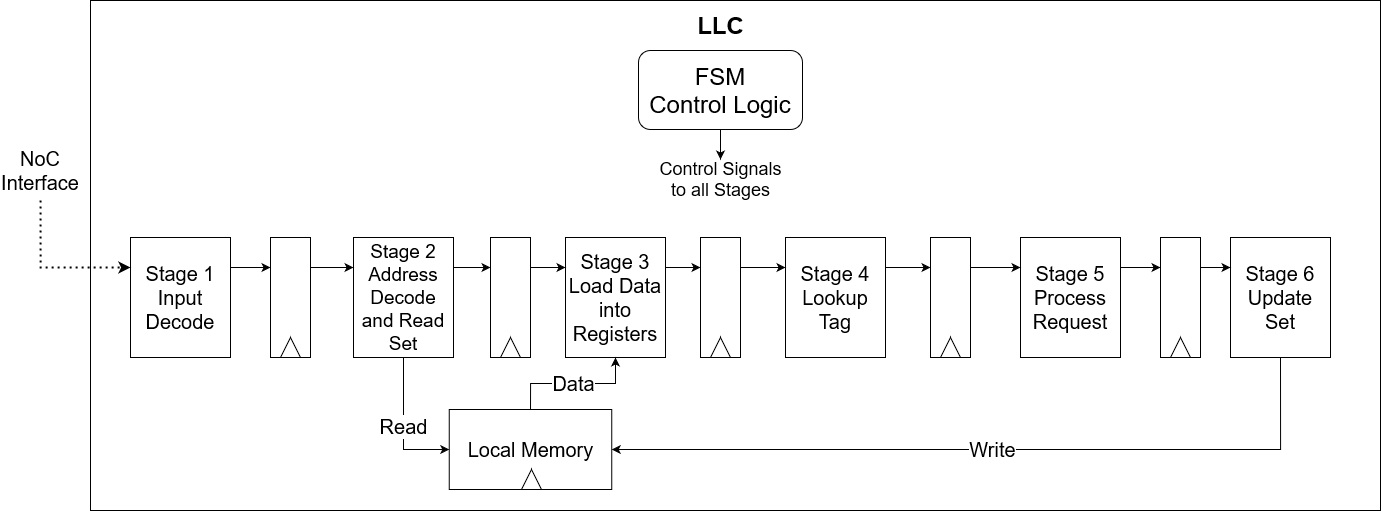
\includegraphics[width=1\textwidth]{fig/LLC_muarc_original.png}
    \caption{Microarchitecture of Original LLC}
    \label{fig:original_muarc}
    \end{figure*}

\begin{figure*}[t]
    \centering
    \captionsetup{justification=centering, format=hang}
    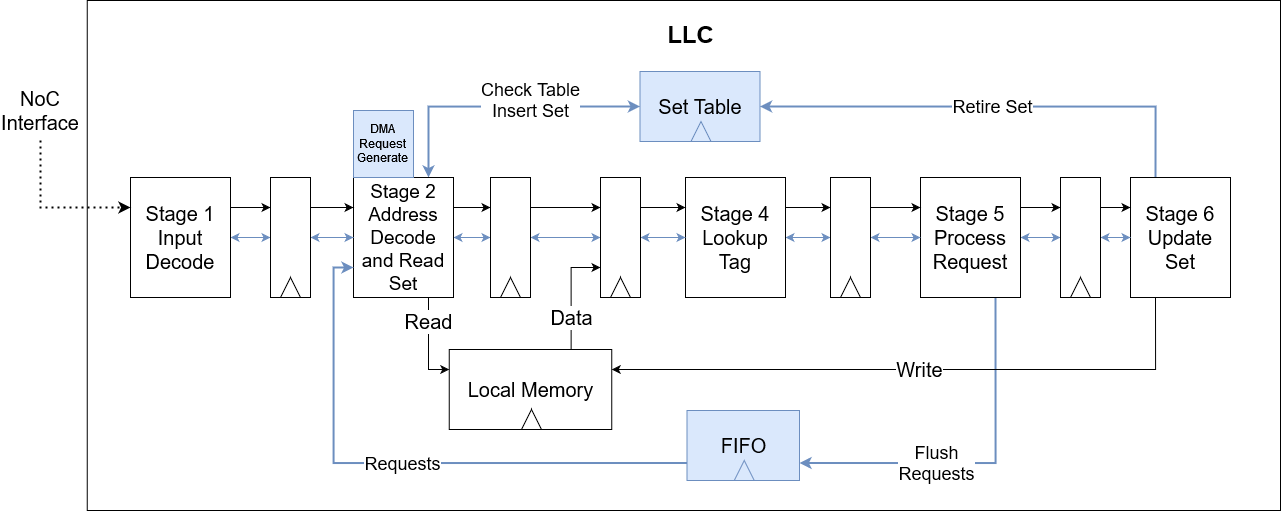
\includegraphics[width=1\textwidth]{fig/LLC_muarc_pipeline2.png}
    \caption{Microarchitecture of Pipelined LLC. Major structural modifications are highlighted in blue.}
    \label{fig:pipeline_muarc}
    \end{figure*}
  
  
